
NIST SP 800-53 \textit{provides a catalog of security and privacy controls for federal information systems and organizations to protect organizational operations and assets, individuals, other
organizations, and the Nation from a diverse set of threats including hostile attacks, natural disasters, structural failures, human errors, and privacy risks.}\cite{Force_2017}

\begin{figure}[H]
\centering
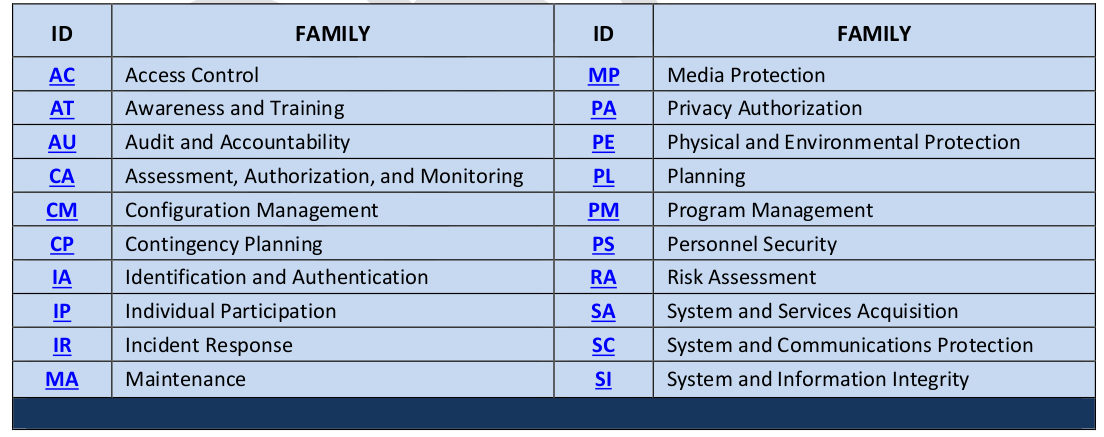
\includegraphics[scale=.4]{img/rmf/800_53_control_fams.png}
\caption{NIST 800.53 Security Control Families \cite{Force_2017}}
\label{fig:800_53_control_fams}
\end{figure}

We have included below the individual controls that would apply directly to TEE implementations during a security review for system accreditation. In most cases the applicable controls would be inherited by any application deployed within the enclave boundary, and we discuss where this may not be the case below. To date we have not studied how to articulate these findings within the RMF\cite{JTF_2018} pipeline, nor have we evaluated the suitability of the publicly available cryptographic implementations against an approved operational standard\cite{Technology_2019}. 



\begin{table}[H]
\centering
\caption{Identification and Authentication}
\label{tab:controls_ia}
\begin{tabular}{@{}ll@{}}
\toprule
IA-1 & Identification and Authentication Policy and Procedures \\ 
IA-2 & Identification and Authentication (Organizational Users) \\
IA-3 & Device Identification and Authentication \\
IA-4 & Identifier Management \\
IA-5 & Authenticator Management \\
IA-6 & Authenticator Feedback \\
IA-7 & Cryptographic Module Authentication \\
IA-8 & Identification and Authentication (Non-organizational Users) \\ \bottomrule
\end{tabular}
\end{table}

Verification of enclave reports is available through Intel's EPID scheme, which allows non-attributable authentication of SGX signatures. Root key material is burned in at the manufacturer through e-fuses. Enclave developers require a certificate issued by Intel for production deployment sealing and attestation. 

\begin{table}[H]
\centering
\caption{Incident Response}
\label{tab:controls_ir}
\begin{tabular}{@{}ll@{}}
\toprule
IR-1 & Incident Response Policy and Procedures \\ 
IR-4 & Incident Handling \\
IR-5 & Incident Monitoring \\
IR-6 & Incident Reporting \\
\bottomrule
\end{tabular}
\end{table}

Access or altering of enclave resources and memory regions are gated by the CPU. Attestation will fail if the enclave report signature is revoked or invalid or if the report contents does not match the expected values. Any alteration of the sealed enclave application will not decrypt. Any attempt to access a loaded enclave by an unauthorized process will trigger CPU access violations. The exceptions we have noted above are in the CPU L3 cache and other shared resources which are susceptible to side channel analysis. 

\begin{table}[H]
\centering
\caption{System and Communications Protection}
\label{tab:controls_sc}
\begin{tabular}{@{}ll@{}}
\toprule
SC-1 & System and Communications Protection Policy and Procedures \\ 
SC-2 & Application Partitioning \\
SC-3 & Security Function Isolation \\
SC-4 & Information In Shared Resources \\
SC-7 & Boundary Protection \\
SC-8 & Transmission Integrity \\
SC-9 & Transmission Confidentiality \\
SC-11 & Trusted Path \\
SC-12 & Cryptographic Key Establishment and Management \\
SC-13 & Use of Cryptography \\
SC-14 & Public Access Protections \\
SC-15 & Collaborative Computing Devices \\
SC-17 & Public Key Infrastructure Certificates \\
SC-18 & Mobile Code \\
SC-23 & Session Authenticity \\
SC-28 & Protection of Information At Rest \\
SC-30 & Virtualization Techniques \\
SC-32 & Information System Partitioning \\
SC-33 & Transmission Preparation Integrity \\
SC-34 & Non-modifiable Executable Programs \\ 
\bottomrule
\end{tabular}
\end{table}

As described above and developed in \cite{sgx-lkl_2018, Priebe_Muthukumaran_Lind_Zhu_Cui_Sartakov_Pietzuch_2019}, terminating TLS endpoints in TEE enclaves prevents communication intercepts when either end of the transmission is untrusted or compromised. Applications are partitioned based on current TCB size limits for performance, although these limits are expected to increase as the technology matures. Cryptography in SGX is pervasive and includes approved implementations, customized proprietary implementations, and everything in between. We are currently formalizing the cryptographic constructs necessary for TEEs to function generally.

\begin{table}[H]
\centering
\caption{System and Information Integrity Policy and Procedures}
\label{tab:controls_si}
\begin{tabular}{@{}ll@{}}
\toprule
SI-1 & System and Information Integrity  \\
SI-3 & Malicious Code Protection \\
SI-4 & Information System Monitoring \\
SI-6 & Security Functionality Verification \\
SI-7 & Software and Information Integrity \\
\bottomrule
\end{tabular}
\end{table}

We have omitted Audit and Accountability \textbf{AU} controls from this list as they are not directly provided by the TEE. However, we are actively developing TEE based secure log streaming capabilities for distributed platforms. The first being an implementation of Apache Metron SOC built on our Storm SGX implementation, and the second is an enclave based sidecar pattern for secure microservice and container logging. Combined these capabilities will provide unalterable evidence trails for active monitoring and incident response.
